\documentclass[onecolumn,10pt]{IEEEtran}

\usepackage{amsmath,amsfonts,amssymb}
\usepackage{graphicx}
%\usepackage{marginnote} % for editorial use
\usepackage{sidenotes} % for editorial use
\usepackage[dvipsnames,svgnames]{xcolor}
\usepackage{svg,svg-extract}
\usepackage{booktabs}

\usepackage{siunitx}
\DeclareSIUnit\foot{ft}
\DeclareSIUnit\pound{lb}
\DeclareSIUnit\ounce{oz}
\DeclareSIUnit\inch{in}
\DeclareSIUnit\rpm{rpm}
\DeclareSIUnit\fahrenheit{F}
\DeclareSIUnit\bit{bit}
\DeclareSIUnit\byte{B}

\newcommand{\myroot}{../}
\newcommand{\Later}{\textbf{Later.}}
\newcommand{\Calypteanna}{\emph{Calypte anna}}
\newcommand{\Canna}{\emph{C.~anna}}
\newcommand{\MATLAB}{Matlab}
\newcommand{\Matlab}{Matlab}

\usepackage{hyperref}
\hypersetup{
  colorlinks=true,
  linkcolor=violet,
  urlcolor=blue,
  citecolor=blue}

\usepackage[plain]{fancyref}
\renewcommand{\freffigname}{Fig.}
\renewcommand{\Freffigname}{Fig.} 
\renewcommand{\freftabname}{Table}
\renewcommand{\Freftabname}{Table}
\frefformat{plain}{\fancyrefeqlabelprefix}{(#1)} 
\Frefformat{plain}{\fancyrefeqlabelprefix}{(#1)} 

\usepackage{listings}
\lstset{
	basicstyle=\ttfamily,
	columns=fullflexible,
	showstringspaces=false
}
\lstdefinestyle{mbedC}{
	language=C,
	basicstyle=\ttfamily,
	keywordstyle=\color{blue}\ttfamily,
	stringstyle=\color{magenta}\ttfamily,
	commentstyle=\color{green}\ttfamily,
	directivestyle=\color{red}\ttfamily,
 	morecomment=[l][\color{red}]{\#},
	columns=fullflexible,
	showstringspaces=false,
%	frame=single
}
\lstdefinestyle{usnaMatlab}{
	basicstyle=\ttfamily,
	keywordstyle=\color{blue}\ttfamily,
	stringstyle=\color{magenta}\ttfamily,
	commentstyle=\color{green}\ttfamily,
 	morecomment=[l][\color{red}]{\#},
	columns=fullflexible,
	showstringspaces=false,
	language=Matlab
%	%backgroundcolor=\color{lightgray},
%	frame=single
}


\title{Autonomous trajectory planning to execute extreme maneuvers based on hummingbird display dives}
\author{MIDN 1/C E.~Marcello and Asst. Prof. D.~Evangelista\thanks{Authors are with the United States Naval Academy, Department of Weapons, Robotics, and Control Engineering}}
\date{\today}


% For EW404 title and signature page
\usepackage{titlepage4956}
\coursenumber{EW404}
\advisor{Assistant Professor D. Evangelista}
\coverpicture{\includegraphics[height=1.88in]{\myroot/figures/problem-statement-1a.png}%
\includegraphics[height=1.88in]{\myroot/figures/problem-statement-1b.png}}


\begin{document}
\maketitlepage
\maketitle

\begin{abstract}
Using a small indoor quadrotor (Crazyflie 2.1), and a multi-camera motion tracking system (OptiTrack) this research seeks to autonomously execute extreme maneuvers observed in flying animals.  My primary goal will be to discover the maximum degree to which a small unmanned aerial system can recreate the courtship display dives of Anna's Hummingbirds (\emph{Calypte anna}) through analysis of a time-scaled root mean square error between the bird and quadrotor trajectories. In animals, and especially in species with sexual selection / female choice, extreme maneuvers are expected to provide an honest signal of mate quality, e.g. his ability to generate large forces and torques and perform fine control during locomotion, including at high speed. Animals also accomplish these in variable environments with varying flow, turbulence, and lighting conditions. Performing such manuevers with unmanned aerial systems is expected to be an engineering challenge that could help provide robotic systems with access to difficult-to-reach places, and further expand their usefulness and applications in the public and private sectors.

%Alt abstract: The research discussed in this paper is concerned with the replication of the highly aggressive aerial maneuvers of the Anna’s Hummingbird on an autonomous quadrotor platform. Specifically, this research aims to determine the extent to which these maneuvers are possible through analysis of a time-scaled root mean square error between the bird and quadrotor trajectories. Analysis will be conducted through both simulation and proof of concept demonstrations on the Crazyflie 2.1 platform. The proof of concept demonstration will utilize an OptiTrack motion capture system to ensure a high degree of accuracy is recorded for the quadrotor trajectory, and the experiment will be conducted inside to minimize any possible disturbances in the air. 

%This research proposal seeks to use aggressive quadrotor maneuvering and path planning to fly the same trajectory Anna’s hummingbirds execute during their courtship display dives with a Crazyflie 2.1 quadrotor. Aggressive autonomous maneuvering for quadrotors has been a focused area of study by many researchers over the past several years; however, there have not yet been many attempts at replicating aggressive flight patterns seen in biological species. In being one of the first research topics into flying Anna’s hummingbird dive trajectories with an autonomous platform, this paper aims to discover an advantage to this specific type of maneuver for autonomous aerial vehicles. To execute this task, I will be relying heavily on prior work completed in autonomous control of the Crazyflie quadrotor, utilizing a quaternion model of the quadrotor flight dynamics. Additionally, I will be using previously obtained data for the Anna’s hummingbird flight trajectories. To measure the feasibility of the maneuver I plan to conduct trials both in simulation and in proof of concept demonstration that will compare the trajectory of the quadrotor to the hummingbird flight trajectory using a root mean square error between sampled data points along the trajectory paths. The total projected cost of the project is \SI{28470}[\$] including a cost \SI{370}[\$] in new materials. The timeline estimates project completion in 24 weeks, with the highest risk being my requirement of learning 2 new programming languages, ROS and Python, and possible damage to the Crazyflie quadrotor in the event of a failed maneuver
\end{abstract}

\begin{IEEEkeywords}
capstone, robotics, controls
\end{IEEEkeywords}


\section{Background and motivation}\label{sec:background}
\IEEEPARstart{A}{nimals moving in a real environment} face many challenges that are currently unsurmountable for typical engineered devices, including small size, difficult-to-achieve power-to-weight ratios, ability to operate in multiple environments, and the ability to control complex maneuvers even in the presence of environmental disturbances such as wind, water flow, or turbulence, variable lighting, or even attack from predators or conspecific rivals. These alone make them worthy of engineering study, but such interdisciplinary work is not a one-way street. 

Biologists may also wish to use engineering to learn how an organism does what it does.  As an example, consider the aerodynamic principles of ``helicopter'' samara seeds such as in maples (\emph{Acer sp.}) and convergently evolved in many other groups.  Samaras are able to slow their descent to the group using a spanwise asymmetric weight distribution and wing structure to facilitate autorotation, allowing them longer hang time during which, on rare occasions, they are swept quite far by a lucky gust of wind. The resulting long dispersal distances are quite advantageous for the saplings, who no longer have to compete with the mother tree. The study of the first autorotating seeds in the fossil record made heavy use of engineering techniques such as autorotation theory, consideration of stability from the vertical separation of the center of gravity and the center of pressure, and nondimensional coefficients governing flight \cite{stevenson2015when}.  As for applications\footnote{Applications of basic biomechanics research may not be immediately obvious, but this is not a reason to ignore biomechanical systems of interest.}, researchers in \cite{who2019maple} developed a monocopter based off of this concept, and were able to develop control algorithms for actively steering such a device. 

Robotic systems are potentially a way to examine form and function in organisms, and organisms are potentially a source of inspiration for improving the robots.  In \cite{feltman2014creepy}, sidewinder-type locomotion, observed in all snakes but most characteristic of the sidewinder rattlesnake (\emph{Crotales cerastes}), was studied by creating a robot to imitate it. In sidewinder locomotion, snakes move across granular media like hot desert sand in a direction lateral to their main body axis; this is accomplished using a combination of body twisting and bending to create moving points of contact with the ground as the body bends.  The robot was developed like a snake, and was programmed to copy as closely as possible the movement of the sidewinder. The initial test had success on level ground, but no such luck on steeper slopes. On closer observation of the live snake, it was discovered that the sidewinder used two independent wavelike motions to move instead of just a single wave. Once this was implemented in the robot, the robot was able to navigate just like the sidewinder, and a new form of ground travel was made attainable by robotic machines. This discovery has applications of movement over a variety of different terrain that a typical wheeled robot would not be able to navigate.

I will be attempting to enhance a quadrotor’s maneuverability by studying the flight patterns and maneuvers of Anna’s Hummingbirds (\Calypteanna), a \SI{5}{\gram} hummingbird native to western North America. Male Anna's Hummingbirds perform a display dive in order to win matings with choosy females. The dive reaches speeds above \SI{27.3}{\meter\per\second} \cite{clark2009courtship}
% \cite{larimer1995accelerational}
 and ends with a 9G pullout maneuver (full 3D field kinematics determined in \cite{clark2009courtship}) culminating in a display of red iridescent feathers on his gorget (throat) and a high frequency tweeting noise made by flow-induced vibration of the distal two retrices (outer tail feathers) \cite{clark2008annas}. Such a maneuver would normally cause G-induced loss of consciousness in a human pilot without a g-suit.  The difficulty of the manuever makes it an honest signal \cite{zahavi1975mate} of mate quality to Anna's Hummingbird females as it requires skill and power to complete. Thus, it is expected to be difficult for a \SI{27}{\gram} quadrotor\footnote{The Crazyflie 2.1 mass is approximately the same as the largest living hummingbird species, the Giant Hummingbird (\emph{Patagona gigas}), native to the Andes.}  to imitate and a worthy challenge. I intend to discover how feasible the dive maneuvers actually are for quadrotors, and explore their operational limits in this respect. 

Unmanned aerial systems are becoming increasingly more autonomous for tasks with position control at comparatively low speeds; a guiding research question is how extreme maneuverability can augment their capabilities by building on previous work in quadrotor control  \cite{mellinger2011minimum, greiff2017modelling}.  The applications of this research are twofold: it will both help in developing a greater understanding of the physical limitations of extreme maneuverability on quadrotors, the primary engineering problem, and it will also provide a greater idea of the effects of such maneuvers on flying animals. The ability to automate the hummingbird dive maneuvers means that other forms of extreme maneuvers might also be autonomously executed, perhaps providing a toolbox or set of skills to use when a UAS is presented with a maneuvering challenge during a mission.  If combined with enhanced sensing abilities, autonomous MAVs would be able to navigate through obstacle-heavy environments with greater speed and ease, allow for evasion or penetration/infiltration, or simplify recovery. 

In addition to this, a successful device could be used in behavioral playback studies in which live hummingbirds are presented with a controllable stimulus mimicking the male display dive.  If a quadrotor were to execute this dive for a female Anna's Hummingbird, could the quadrotor generate a favorable response from her? If so, it may be possible to alter the pattern to present a super-normal stimulus or probe which aspects of the display are most appealing to her.  Such a study in hummingbirds would be novel\footnote{von Frisch, Lorenz, and Tinbergen won the 1973 Nobel Prize for Physiology or Medicine for ``discoveries concerning organization and elicitation of individual and social behaviour patterns...'' among other things, including use of robots to examine honeybee dance language and supernormal stimuli in herring hull beak markings.}  as biologists have not been able to produce the maneuvers themselves.
 %\section{Background and motivation}
\section{Problem statement}
I aim to execute aggressive maneuvers similar to the display dives of male Anna’s Hummingbirds (\Calypteanna) with an autonomous quadrotor platform. 

My project assumes the following are provided: a quadrotor and  flight controller (e.g. Crazyflie 2.1, Bitcraze, Malm\"{o}, Sweden), and a method of obtaining three-dimensional (3D) position data of the quadrotor in test flights (e.g. OptiTrack, NaturalPoint Inc., Corvalis, OR). Example trajectories obtained from live hummingbirds will be obtained from \cite{clark2009courtship}.  Given a desired hummingbird flight trajectory, depicted in \fref{fig:problem-statement-1}a, the system will autonomously generate and execute the control inputs required to successfully complete the maneuver. 

A successful maneuver is defined as a root mean square error (RMSE) calculation of less than \SI{10}{cm} between the time-scaled hummingbird trajectory and the quadrotor trajectory, with a standard deviation $\sigma$ of \SI{5}{cm} over the entire dataset. The RMSE will be calculated between the $x$, $y$, $z$ position data for each pair of data points that share the same time value, $t$. The hummingbird trajectory will be scaled by a constant factor in time to allow for the physical limitations of the quadrotor--e.g. the quadrotor may only have to travel the desired trajectory at half the speed of the hummingbird to still achieve a successful maneuver. The hummingbird trajectory will also be geometrically dilated to a smaller overall trajectory path in order to physically fit the trajectory inside the available lab space. These are necessary adaptations due to the impressive speed and acceleration capabilities of the Anna’s hummingbirds relative to their size \cite{clark2009courtship}, and of course the physical size constraints of the Maury 201 labroom. 
\begin{figure}[h]
\begin{center}
\includegraphics[height=1.88in]{\myroot/figures/problem-statement-1a.png}%
\includegraphics[height=1.88in]{\myroot/figures/problem-statement-1b.png}
\end{center}
\caption{(a) The five stages of an Anna’s Hummingbird dive maneuver, from \cite{clark2009courtship}. (b) A quadrotor using path planning to fly through a thrown hoop, from \cite{mellinger2011minimum}.}
\label{fig:problem-statement-1}
\end{figure}

As a stretch goal, I will also analyze and replicate a variety of different types of hummingbird dives and maneuvers, to include evasive aerial maneuvers \cite{sholtis2015field, cheng2016flight}. Success will be determined in the same fashion as described above. %\section{Problem statement}
\section{Literature review}
\label{sec:literature}

%The inspiration of this project proposal has its roots in the high maneuverability seen by hummingbirds. As such, it was essential to be able to gather data on hummingbird trajectories in order to study their feasibility of being replicated by a quadrotor. There have been many bio researchers that have delved into the study of hummingbirds, however I will mainly discuss the works \cite{clark2009courtship} and \cite{cheng2016flight}. 

The work in \cite{cheng2016flight} determined the trajectory and body kinematics of four different hummingbird species in an evasive maneuver. This was done by startling the birds while they were hovering, and observing their movements with three high definition cameras to provide a 3D position \cite{hedrick2008software, theriault2014protocol, jackson20163d}. Birds were marked with water-soluble white paint to ease digitization and tracking. I will use a similar optical tracking methods as in \cite{cheng2016flight, hedrick2008software, theriault2014protocol, jackson20163d}, with the added simplifications of being able to install known, infrared (IR) relfective markers for automatic tracking and using a RANSAC algorithm to estimate pose. In addition, the evasive maneuvers studied in \cite{cheng2016flight, sholtis2015field} could be useful for quadrotors attempting to avoid capture or a counter-UAS drone denial system (e.g. USNA Project Midknight or similar).

% Water-soluble white paint was used to make dot markings on the hummingbird’s body to help model the wing and head positions for each trial. The data they acquired in their experiments includes many more details than I will need to use, however they provide data on the hummingbird’s velocity and trajectories for several trials which I can use to help develop my quadrotor trajectories. , they and I will both be using optical data to obtain a position fix. With regard to the type of maneuver that these birds are required to perform, it aligns well with the type of experimentation that I aim to work with. Evasive maneuvers are certainly a type of extreme maneuver, and these patterns may prove to be something that I wish to try on my quadrotor. Evasive maneuvers can be useful for quadrotors if they are in threat of being netted, and if I am able to copy the hummingbird’s trajectory, further analysis and testing may prove that this type of trajectory provides a maneuvering or sensing advantage to the quadrotor in evasive flight.

The work in \cite{clark2009courtship} obtained fully 3D field kinematics of courtship dives in \Canna\ in order to study extreme locomotor performance in animals. \cite{clark2009courtship} used multiple calibrated high speed cameras and manual digitization to reconstruct the birds' 3D position during dives.  Splines were used to estimate acceleration and velocity from positions without undue amplification of noise. \cite{clark2009courtship} also examined wing and tail movements and sounds produced during dives.  As a measure of the biomechanical difficulty of the maneuver, \cite{clark2009courtship} estimated the maximum stresses in the humerus during dive pullout; such a quantity would be extraordinarily difficult to measure \emph{in vivo} but in  my work there is a possibility of directly instrumenting the quadrotor to examine forces, torques, stresses, and engineering limits. 
%Again, this is more detailed data than I will need for trajectory replication on my quadrotor. This paper gives an insight into what exactly I will be trying to achieve through the extreme maneuverability of my quadrotor. Since this type of maneuver is estimated to cause a lot of strain on the hummingbird, it is likely to also cause a lot of strain on a quadrotor. Through simulation and proof of concept demonstration, I will be able to provide a more accurate picture of just how difficult these maneuvers can actually be.

After obtaining these hummingbird trajectories, an effective method of modeling a quadrotor and conducting trajectory planning is required. In \cite{tomic2014learning}, the authors developed metrics and constraints for quadrotor maneuvering performance and a machine learning workflow. This was achieved through the solving of an optimal control problem offline, and then using a machine learning technique to learn these trajectory solutions with the given constraints. The result was then used to develop online solutions  for near-optimal trajectories for a quadrotor. This was done in the $x$-$z$ plane for point to point and perching maneuvers, as well as joint trajectories. To validate their solution, they flew these optimal trajectories using both Simulink simulations, and proof of concept demonstrations. Since I will be using a quadrotor platform, this paper directly applies to my problem statement as a good reference base that I can use to springboard my exploration into more complex extreme maneuvering. The basis of this work will give me a much more quantitative measure of success in terms of how close my developed trajectories are to an optimal path. \cite{tomic2014learning} is very thorough and provides a clear distinction and improvement on previous work in quadcopter trajectories, especially with regard to the joint trajectory problem. I can build on this by expanding into 3D trajectories instead of just working in a 2D plane, and I can also try to utilize their proxy-based joining method to create a desired path curvature.

In \cite{sabatino2015quadrotor}, the authors developed a linearized model of a quadrotor in planar motion. The careful process by which the quadrotor dynamics are identified and modeled will be helpful in my own research as I develop my own model for the quadrotor that I will be using. In \cite{sabatino2015quadrotor}, their modeling method is done for three different linearization methods and each of these is compared to each other by running a Simulink simulation with each controller. Quantities compared include several attributes of the step response, and the actual trajectory of the quadrotor compared to the desired trajectory. This comparison method between the different trajectories is similar to the validation work that I will need to do on my own simulation. As such, this work will help me to better understand ways of determining the accuracy of my trajectory testing in simulation, and in proof of concept demonstration. This paper, while a good starting point for my work, does not attempt to go into more complex maneuvers. These are discussed in greater detail in the following works.

In \cite{liu2017planning}, the development of trajectories and path planning for UAVs was accomplished. They did this by determining the maximum overload, minimum turn radius, and maximum flight endurance of the experimental quadrotors in order to come up with feasible aggressive trajectories. Trajectories had the constraint that they had to follow a sixth order (or lower) polynomial trajectory. Much like my proposed concept, this work develops an attitude and trajectory controller with appropriate initial and final conditions, as well as a boundary “tube” which the quadrotor must stay within for every trajectory. The work in this project is heavily relevant to my proposed work, as they achieve a working simulation of aggressive trajectories with their path-planning algorithm and onboard controllers. I would like to expand on this work by flying a shorter trial with hummingbird-like flight patterns. 

Finally, \cite{mellinger2011minimum} offers some of the closest work to exactly what I am proposing for my own work. The main focus of this paper is to create trajectories for quadrotors in real time in an indoor or constrained environment. They also pay particular attention to the velocity and acceleration vectors of the quadrotor throughout its maneuver. I will also need to be able to achieve these types of measurements from my system, and be able to change my controller to affect them in an appropriate manner in order to fully achieve a trajectory flight path that replicates a hummingbird maneuver. \cite{mellinger2011minimum} also uses temporal scaling to fly their trajectories at different speeds, which is exactly what I will need to do when and if I find that flying the hummingbird trajectory at full speed is either not possible or extremely dangerous. 
 %\section{Literature review}
\section{Materials and methods}
\label{sec:methods}

To demonstrate the objective of replicating \Canna\ display dives,  I simulated the system in \MATLAB\ and Simulink.  This was to be followed up with a proof-of-concept demonstration, provided I am able to achieve successful trials in simulation first; however, the demonstration was affected by the global COVID-19 pandemic. Simulation was used because it was more general and allowed easy changing of parameters and control methods to more completely explore the space; simulations also allowed examination of behavior at actual hummingbird flight speeds without risking excessive damage to the hardware. Simulations make simplifying assumptions by necessity, so actual testing and demonstration using real quadrotors--namely the Crazyflie 2.1--were also planned. Unfortunately, due to the inaccessibility of hardware brought about by the stay-at-home orders issued by the DoD in March of 2020, a final hardware demonstration of trajectory flight was never executed. Progress made towards achieving a hardware demonstration is described later in this report.  
% This part is way too wordy and non-sequitur. 
%Before I describe these processes, it is important to mention why these are the methods I chose to implement. A simulation is general in that I can run the simulation for many iterations to see how the controller will react to different input parameters. The input parameters themselves are very specific; however, the ability to change parameter values will allow me to assess the full capabilities of the quadrotor system to determine if I can eliminate the need to do a time-scaled comparison to the hummingbird trajectory. The simulation will be coded using MATLAB and Simulink, both are software with which I have the most experience in creating simulations. My simulation code will be made available after the completion to this project on Git for those wishing to replicate my simulated results. Unfortunately, the realism of this simulation is limited, and as a result I will have to do a proof-of-concept demonstration to truly prove the ability of the quadrotor. Being a much more specific process, it will likely vary slightly from the simulation results, and need to be tweaked based on the level of success seen in the first few trials. Ultimately, the proof-of-concept demonstration is an essential piece to this research since a simulation doesn’t have any real world application except in principle. The experiment will enlist the use of a Crazyflie quadrotor platform, and an OptiTrack motion capture system in order to gather position vs. time data. This will help ensure accuracy in the quadrotor’s trajectory and as such, provide a higher level of confidence in the experiment’s success.

For my concept demonstrations, I modeled the rigid body dynamics of the quadrotor using parameters obtained from the Bitcraze website\footnote{\url{https://wiki.bitcraze.io/misc:investigations:thrust}}, and distance measurements taken by calipers. For initial attempts at control, the hover condition was assumed. This is a control linearization region which assumes the attitude of the quadrotor is completely level, i.e. the pitch and roll angles are assumed to be approximately zero degrees during all stages of flight. A basic waypoint position controller was utilized first in order to ensure controller functionality in simulation and on the hardware itself. A PD controller was used initially for position control, as this is a ubiquitous controller well understood by students and control theorists. Initial gains were taken from the simulation \cite{hartman2014quadcopter}
%cite dch33/Quad-Sim on github (this is the 2014 one from hartman cited here) LINK: https://github.com/dch33/Quad-Sim 
 and later adjusted to fine-tune the quadrotor response. Additionally, in order to avoid an excessive attitude command in the event of large position errors, saturation limits were be placed on the attitude command of \ang{\pm 45} in order to ensure the quadrotor doesn't over-rotate and accidentally flip over. 

The functional block diagram of the overall Crazyflie control system is shown in \fref{fig:demonstration-2}. The laptop is the central node in the control scheme, obtaining position and orientation information from the OptiTrack system, and then relaying this data to the Crazyflie in addition to the next desired position on the trajectory path. The Crazyflie then conducts onboard error calculation and command processing in order to control its position in 3D space.

% the quaternion model in \cite{greiff2017modeling}. A quaternion is defined as 
%\begin{equation}
%Q = a + b i + c j + d k
%\end{equation}
%where $i$, $j$, and $k$ are imaginary unit vectors. This model also assumes a right-handed coordinate system where $i\cdot j = k$ , and the fundamental assumptions hold true -- i.e.  $i^2 = j^2 = k^2 = ijk = -1$.  I have chosen to use this model due to the limitations of the Euler model at high rotation angles. The quaternion model will be robust to these extreme angles, and is therefore better suited for my experiment. \emph{\textbf{Evangelista comment here: this is sort of strange to mention here. It's like saying I plan to use math, or matrices, or eigenvalues. Choosing to represent rotations as quaternions is a useful thing for avoiding gimbal lock associated with singularities in the Euler angle representation, but would not be considered a defining characteristic of what you plan to do, more like a low level design choice comparable to what units you use, or if you like floats or doubles.}}

\subsection{Simulation of bio-inspired dive pullout maneuvers in \Matlab}
%To create a feasible simulation for this research, I will model the Crazyflie quadrotor platform to be used in simulation. This involves determining the various thrust vectors of the motors, and the calculation of many performance metrics. Thankfully, much of this work has already been done, and I will be relying heavily on the work in \cite{cheng2016flight} to create a useful model for the quadrotor in \MATLAB\ and Simulink.
% Due to the extreme maneuvering of the quadrotor, I have chosen to use a quaternion coordinate system to describe its position, for flight control purposes only. %A quaternion is defined as a vector of one real and three imaginary vector directions, $i$, $j$, and $k$.

Using the model of the Crazyflie quadrotor described in the \lstinline{PC_Quadcopter_Simulation.slx} \MATLAB\ Simulink simulation \cite{hartman2014quadcopter}, 
%cite quadsim_68
and hummingbird trajectory data obtained from \cite{clark2009courtship}, several trajectory comparisons were conducted in the $x$, $y$, $z$ Cartesian coordinate frame between the true hummingbird trajectory (desired trajectory) and the actual flown trajectory by the simulated Crazyflie. Since the dive trajectories have little deviation in the $y$ coordinate axis, they are compared only in the $x$ and $z$ axes for all relevant error calculations. 

%I added the following bit to explain the initial conditions, but if it's too wordy or doesn't make sense here it should be moved to a spot where it makes more sense to explain this concept.
Simulations were conducted from two different initial quadcopter states. The first simulation was run with the quadcopter starting from rest on the ground. This requires the quadcopter to ascend to the top of the trajectory first and then begin the trajectory flight, which simulates what I would have to replicate for the hardware demonstration. The second initializes the quadcopter at the beginning of the hummingbird trajectory, with an initial velocity determined by calculating the instantaneous velocity of the second data point $\delta x/\delta t$, and $\delta z/\delta t$ (both $x$ and $z$ directions) of the original hummingbird trajectory, where $\delta x = x(t = t_1) - x(t = t_0)$. These velocities were then multiplied by a scale factor based on the simulation speed (e.g. the initial velocities were reduced by a factor of 20 for a simulation trajectory at 20 times reduced speed) in order to maintain a realistic starting velocity at each of the different trajectory speeds.
%end of initial conditions spiel
%The feedback diagram of this control concept is shown below in \fref{fig:demonstration-2}. In principle, a desired trajectory will be developed from a path-planning algorithm that takes in the time scaled hummingbird trajectory and calculates the idealized pitch and motor torque and speed at each time step in order to fit this trajectory with as little error as possible. This signal will be combined with some sort of inertial measurement true position feedback to produce the error signal to the onboard flight controller. The flight controller will send a signal to the motors on the quadrotor based on this error signal to come as close as possible to zero error for the next time step, and the cycle will repeat until the quadrotor has completed its maneuver. My simulation will replicate this decision-making process using numerical integration to obtain the position data for every iteration.

%this figure needs to be moved but I'm not sure how. It's printing well above the section that it's listed in here. add a [h] (for here) or move the figure around where it is in the code. 
\begin{figure}[h]
\begin{center}
\includegraphics[width=0.8\columnwidth]{\myroot/figures/FunctionalBlockDiagram_system.png}
\end{center}
\caption{Functional block diagram of the data communication flow concept for the autonomously controlled Crazyflie, with an included onboard controller feedback loop.}
\label{fig:demonstration-2}
\end{figure}

To determine the accuracy of the trial I compared the actual flight path of the quadrotor with the desired flight path, and determined a time-scaled root mean square error between the two position vs time datasets. This error was calculated using the distance formula \fref{eq:demonstration-1}:
\begin{equation}
e_p(t) = \sqrt{(x_a(t)-x_d(t))^2 + (z_a(t)-z_d(t))^2}
%\begin{bmatrix}
%x(t) \\ y(t) \\ z(t)
%\end{bmatrix}_a^2 
%-
%\begin{bmatrix}
%x(t) \\ y(t) \\ z(t)
%\end{bmatrix}_d^2
%}
\label{eq:demonstration-1}
\end{equation}
where $e_p(t)$ is the position error at a specific time step (time $t$) in the trajectory, and the subscripts $a$ and $d$ represent the actual traveled trajectory and the desired trajectory respectively. The error in the $y$ axis is omitted since the trajectory is 2D in the $x$-$z$ plane and errors in the $y$ axis are therefore negligible for a stable controller, as is assumed. The error for every time step was averaged together to determine the root mean square error of the data. Additionally, the standard deviation $\sigma$ of the position error was calculated using the \lstinline{std()} function in \MATLAB. Without any other indications, a successful trial was considered to be one with root mean square error of less than \SI{10}{\centi\meter} over the entire trajectory, and with a $\sigma$ value of less than \SI{5}{\centi\meter}. Since the hummingbird trajectory is time-scaled down to only a fraction of its true speed, the quadrotor onboard controller was responsible for marking every position at the time it is supposed to be located at that position, therefore limiting the effects that motor operation constraints, e.g. thrust saturation, as a possible source of error in the trajectory flight.






\subsection{Tuning controller gain} %TALK HERE ABOUT CONTROLLER GAIN TUNING METHODS
After the initial simulation runs, I anticipated large position errors over the trajectory flight. As such, it was desirable to tune the control gains in order to achieve a lower root mean square error. The simulation consists of two separate levels of control. The first level is a high-level (outer loop) PD controller concerning the $x$ and $y$ position of the quadcopter, and the second level is the lower-level (inner loop) PID controller that actually determines the pitch and roll angle of the quadcopter, as well as its vertical ($z$) position. The first level is a path planning step carried out among the Optitrack (sensor), control computer, and the drone.  The second level is flight stabilization (auto mode) carried out by the flight controller native onboard the drone. The output of the first level controller is factored as input into the second level controller, along with the quadcopter state. Separate control gains are used for each degree of freedom, i.e. the control gains for the pitch angle of the quadcopter are completely independent of those for the roll angle, altitude, yaw angle, etc. In all, there are eight different control gains that characterize the behavior of the quadcopter through the 2D $x$-$z$ hummingbird trajectory: the proportional and derivative control gains for the $x$ position ($K_{px}$, and $K_{dx}$), and the proportional, derivative, and integral control gains for both the pitch $\theta$ and altitude $z$ $($respectively, $K_{p\theta}$, $K_{d\theta}$, $K_{i\theta}$, $K_{pz}$, $K_{dz}$, $K_{iz}$). 

In general, the effects of changing the proportional control gain will increase the responsiveness of the system with regard to the parameter effected by the controller. As the proportional gain is increased, overcontrolling is noted as oscillations around the desired state grow with a continued gain increase. An increase in the derivative control gain will help to counterbalance this effect to improve the overall stability of the system and reduce overshoot, while an increase in the integral control gain will reduce/eliminate oscillations around the desired settling state, bringing the steady state error to zero. As such, with regard to the effect of the control gains on the simulation output, I expect that increasing both the proportional and derivative gains should help to quicken the response of the quadrotor, and achieve a smaller root mean square error when flying the desired trajectory while remaining stable.


\subsubsection{Manual gain tuning}
Several methods of gain tuning were attempted, with varying levels of success, to reduce the root mean square error of the quadrotor flight. These methods include manual gain tuning, nonlinear optimization routines, and marginal analysis. Manual gain tuning was attempted first. Initially, the proportional gain was increased separately for each of the three characteristic control loops ($x$, $z$, and $\theta$) until signs of overcontrol/instability were noticed in the response (mostly by large oscillations around the desired control point). Then the derivative control gains were increased for each of these controllers to quell the unstable oscillations. Manual gain tuning was successful at reducing the root mean square error, and the detailed/numerical results are recorded in the Results section of this report.

\subsubsection{Attempted optimization using \lstinline{fmincon}} 
After the manual gain tuning was unable to achieve the desired performance for the quadrotor, I began looking into different ways to attempt to optimize the controller gains to achieve a minimum root mean square error. I decided to use the \MATLAB\ function, \lstinline{fmincon()} to optimize the controller gains, which finds the minimum value of a constrained nonlinear multivariable function through an iterative process. Before attempting to use the function for my problem, I completed the example problem listed in the \MATLAB\ documentation for \lstinline{fmincon()} to minimize Rosenbrock's function. This test allowed me to orient myself with using the \lstinline{fmincon()} tool, and helped to build my objective function for use on my simulation. 

In defining my optimization problem, the eight characteristic control gains ($K_{px}$, $K_{dx}$, $K_{p\theta}$, $K_{d\theta}$, $K_{i\theta}$, $K_{pz}$, $K_{dz}$, and $K_{iz}$) are the decision variables, using the values I had determined during my manual gain tuning as the initial point $x0$. My output variable (what I'm trying to optimize) is the root mean square error between the desired and actual trajectory flown by the quadcopter in the simulation. My objective function was the piece that was a little less straightforward, as it required multiple lines of \MATLAB\ code to achieve. I first set up the appropriate simulation parameters based on the changes to the decision variables made by the \lstinline{fmincon()} optimization routine. Then, I ran the simulation for a set time of 20 seconds to allow sufficient time for the quadcopter to complete the trajectory flight. Following this, I had to determine the start and end points of the trajectory flight. The start point was simply the first index of the simulation output, since the quadcopter started at the top of the trajectory. The endpoint was determined by the index of the output where the commanded position at that index was the exact same as the commanded position two iterations after that point. (The simulation continues to command the last timeseries position provided by the input until the simulation time runs out, therefore a repeated position command in adjacent time steps means that the dive trajectory has ended.) Once the starting and ending index of the simulation output were determined, I was then able to use the error calculation described by \fref{eq:demonstration-1} to determine the root square error of each time step, and average these values to find the root mean square error, completing my objective function.

In my first attempts at running the optimization routine I left the decision variables only constrained by the basic requirement that they had to be nonzero and positive. The optimizer would complete the first iteration at the initial point with no problems, but as soon as it changed the gains for the second iteration, it caused the system to become unstable and the simulation crashed with multiple zero-crossing errors. In attempts to remedy this, I changed several different simulation settings to ignore zero crossing errors and change the simulation step size, all to no avail. I then tried to add constraints to the upper bound of the decision variables (they were already constrained on the lower bound to be greater than zero), in an attempt to prevent the simulation from becoming unstable while \lstinline{fmincon()} tweaked the control gains. This was successful in that the optimization routine was able to run its course; however, the result only made small changes to the initial control gains (less than a tenth of a percent change) which resulted in no significant effect on the output variable, the root mean square error. The simulation is therefore seemingly unable to support optimization routines as it is currently written.

\subsubsection{Marginal analysis... when optimization failed}
After the attempt at control gain optimization proved unsuccessful, I decided to conduct a marginal analysis in order to determine which variables would contribute most to the reduction of the root mean square error. A marginal analysis test simply makes a small change to a decision variable, and then records the overall benefit gained and cost incurred from making that small change. Running this analysis provides insight into how this current controller scheme could be tuned further to achieve greater success at flying the quadcopter through the desired trajectory. I again used the gain values obtained from manual tuning as my initial point, and wrote a \MATLAB\ script to iterate through each gain value and run the simulation on three separate cases for each: a run with the gain at the initial point, a run with the gain decreased by 5\%, and a run with the gain increased by 5\%. After each simulation, error data was collected and saved for processing. 








\subsection{Demonstration of bio-inspired dive pullout maneuver using Crazyflie quadrotor}
Hardware implementation is essential to verifying that the findings of the simulation are accurate. The path to a successful hardware demonstration was a multi-step process. We needed to test the capability of the crazyflie to operate under manual control, open loop control, and then finally introduce closed-loop control of the crazyflie using an optical motion tracking system. As such, the hardware components necessary for this experiment include a fully functional Crazyflie quadrotor (Bitcraze, Malm\"{o}, Sweden), and an OptiTrack system (NaturalPoint Inc., Corvallis, OR). The quadrotor will be the object of the experiment, and the OptiTrack system serves as a highly accurate way to obtain position data for the Crazyflie in flight. It achieves this using visual information from nearly 20 cameras staged around the outside of the testing area. Initial experimentation will be conducted indoors to minimize any aerodynamic noise, although future trials could test controller robustness by introducing environment disturbances. Several batteries for the Crazyflie are needed to ensure sufficient trial and testing periods, and approximately five OptiTrack visual markers must be affixed asymetrically\footnote{This is to clearly distinguish the rigid body axes relative to the markers to ensure proper pose readings.} on each Crazyflie drone to ensure that it is able to be detected by the OptiTrack system and that its state is measured appropriately. These marker additions will be taken into account in simulation first in order to ensure readiness to counteract any effect they may have on the dynamics of the quadrotor in the feedback loop.

As an initial test of hardware, I used the \lstinline{cfclient} software (Bitcraze, Malm\"{o}, Sweden; \url{https://github.com/bitcraze/crazyflie-clients-python}) to link to the crazyflie from a linux machine, and test manual control of the crazyflie using a Logitech USB gamepad (Logitech F310; Lausanne, Switzerland) and a Crazyradio sending velocity and thrust commands to the Crazyflie. This allowed me to gain a basic understanding of how the crazyflie communicated with the linux machine over radio control, and how this might be implemented in a python script. I then tested the motion tracking system capabilities by obtaining automatic 3D position tracking data via the OptiTrack. The OptiTrack system worked independently from this workstation, and recorded $x$, $y$, $z$ position data while logging the time $t$ that each data point was recorded at. 

%The Crazyflie was controlled manually, from a computer, using the bitcraze \lstinline{cfclient} software (Bitcraze, Malm\"{o}, Sweden; \url{https://github.com/bitcraze/crazyflie-clients-python}). To establish manual flight control, the computer was equipped with a USB gamepad (Logitech F310; Lausanne, Switzerland) and a Crazyradio sending velocity and thrust commands to the Crazyflie. The OptiTrack system worked independently from this workstation, and recorded $x$, $y$, $z$ position data while logging the time $t$ that each data point was recorded at. 

%DISCUSS FURTHER HARDWARE DEMONSTRATION HERE. HURDLES, ETC. FIND INFO IN PROGRESS FILE ON DRIVE
%In simulation, we observed that as the speed of the maneuver increased, it was more difficult for the crazyflie to fly it accurately. We wanted to test the same trajectories on hardware in order to see if the actual crazyflie would behave in a similar manner (show a similar error in trajectory flight flying at the same speeds tested in simulation). 

%NOTE: THE TeX compiler doesn't like underscores, and won't compile if you have a naked one in the text. To solve, just put a '\' in front of it and it will render the underscore '_' as just text and will compile just fine.
The next step towards a full hardware demonstration was to test autonomous control of the Crazyflie. To support this, I cloned the \lstinline{whoenig/crazyflie_ros} github repository (\url{https://github.com/whoenig/crazyflie_ros}) which utilizes a ROS framework to run multiple python and C++ scripts that send appropriate commands to the Crazyflie based on the tasking in the files that are run. The demo package of the repository contained a plethora of different example scripts and launch files that would provide the capability needed to complete the hardware testing that I desired, including options for manual joystick control, open-loop hovering control, and closed-loop control using both Vicon (Vicon Motion Capture; Oxford, UK), an optical motion tracking system, and VRPN connection to an alternate motion tracking system such as OptiTrack (Optitrack; Corvallis, OR). I progressively ran through several of the lower level control demo packages, testing first manual control with the USB gamepad using ROS, followed by open-loop control (which ultimately resulted in the Crazyflie crashing into the ceiling due to no closed-loop feedback). Through adaptation of the vrpn control demo scripts, I was able to achieve a successful implementation of a closed-loop hover at a desired 3D location. This worked similar to waypoint control, but only consisting of two waypoints (i.e. the starting and ending point). This meant that waypoint trajectory flight would be possible in the Maury lab with the provided controller. 

Unfortunately, due to the global COVID-19 pandemic, this was as much as I was able to achieve in terms of a hardware demonstration of capability. My work up to this point has been saved in a github repository (\url{https://github.com/devangel77b/marcello-2020-code}), and should be easily accessible and run-able by any student wishing to use the combined Crazyflie OptiTrack system to conduct waypoint flight hardware demonstrations. I have also left fairly detailed instructions in a Google document, which is available on the \lstinline{marcello-2020} Google Shared Drive.
 %\secton{Methods and materials}
\section{Results}
\label{sec:results}

Code and data are available at the Github repostitories here: \url{https://github.com/devangel77b/marcello-2020-code} and here: \url{https://github.com/devangel77b/marcello-manuscripts}. 

\subsection{Initial simulations of bio-inspired dive pullout maneuvers in \Matlab}
%if possible, add a sub-sub section for results
Using the modeling framework of \cite{hartman2014quadcopter}, four trials were run at varying speed reductions: a trial run at the actual hummingbird trajectory's speed, a trial at one fifth the hummingbird trajectory's speed, a trial at one tenth speed, and a trial at one twentieth speed relative to the full scale, full speed trajectories in \cite{clark2009courtship}. The results of those tests are shown in Figs.~\ref{fig:actualspeed}-\ref{fig:onetwentiethspeed}. Distance error calculations for the four trials are shown in \fref{tab:RMSE}. 
%reference the 4 trajectory path figures from actual speed to one twentieth
%why is this so not in the right place
%It also should be LARGER if at all possible. It's kind of tiny which makes it difficult to read
%Larger is tough - this is actually right size it should be same size font as text..normalyl would fit inside a column. 
\begin{table}[hb]
\caption{Distance error calculations for each trial (actual speed, one fifth speed, one tenth speed, and one twentieth speed). RMS position error, combining $x$ and $z$, is represented by the variable $e_p$, defined in \fref{eq:demonstration-1}.}
\label{tab:RMSE}
\begin{center}
%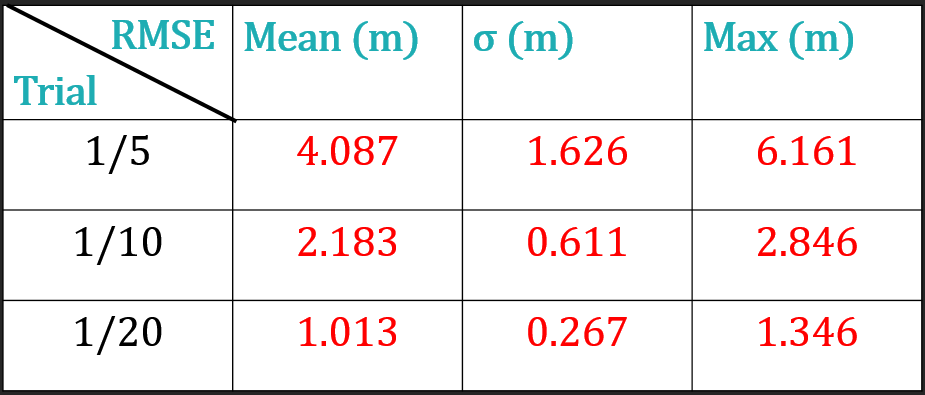
\includegraphics[width=0.6\columnwidth]{\myroot/figures/RMSEtable.png}
\begin{tabular}{cccc}
\toprule
Trial & $\overline{e_p}, \si{\meter}$ & $\sigma_{e_p}, \si{\meter}$ & $\max(e_p), \si{\meter}$  \\ %want absolute value bars or cap X to indicate a multi-dimension magnitude error and not only in the x direction --seems clear without, uglier with bars and e_p is defined before
\midrule
1 & 6.6888 & 4.3926 & 13.5984 \\
1/5 & 3.9415 & 1.8710 & 6.3231 \\
1/10 & 2.1757 & 0.7700 & 2.9967 \\
1/20 & 1.0443 & 0.3328 & 1.3603 \\
\bottomrule
\end{tabular}
\end{center}
\end{table}

For these experiments, the attitude angle command saturation limits were increased to $\pm\ang{45}$ to allow for larger command inputs to take advantage of a wider range of pitch angles. The simulated quadrotor was able to follow the one twentieth speed reduction the closest, and had the smallest RMSE, while the trial at one fifth the speed was incredibly behind the desired trajectory path. The trial at normal speed showed how inferior this control method is at executing high-speed extreme maneuvers, as the quadrotor was barely able to begin accelerating by the time the simulation called for the quadrotor to be completing the trajectory. As such, further experimentation with this controller at actual speed was discontinued, as it seems more relevant to focus on improving the control at slower speeds first before attempting improvment at full speed.

\clearpage
%These figures aren't showing up in subsection A like I want them to.....
%Figures here!!!! (4) with captions
% [p] makes it want to put it on a page of floats, so either clear a page to put them on
% or make them a little smaller
\begin{figure}[p]
\begin{center}
\includegraphics[width=0.6\columnwidth]{\myroot/figures/traj_1x.png}
\end{center}
\caption{Crazyflie attempted trajectory flight of the hummingbird trajectory at its actual speed.}
\label{fig:actualspeed}
\end{figure}

\begin{figure}[p]
\begin{center}
\includegraphics[width=0.6\columnwidth]{\myroot/figures/traj_5x.png}
\end{center}
\caption{Crazyflie attempted trajectory flight of the hummingbird trajectory at one fifth its actual speed.}
\label{fig:onefifthspeed}
\end{figure}

\clearpage
\begin{figure}[p]
\begin{center}
\includegraphics[width=0.6\columnwidth]{\myroot/figures/traj_10x.png}
\end{center}
\caption{Crazyflie attempted trajectory flight of the hummingbird trajectory at one tenth its actual speed.}
\label{fig:onetenthspeed}
\end{figure}

\begin{figure}[p]
\begin{center}
\includegraphics[width=0.6\columnwidth]{\myroot/figures/traj_20x.png}
\end{center}
\caption{Crazyflie attempted trajectory flight of the hummingbird trajectory at one twentieth its actual speed.}
\label{fig:onetwentiethspeed}
\end{figure}








% THE FOLLOWING IS NEW WORK DONE  ON GAIN TUNING AND RESULTING ERROR IMPROVEMENTS
\clearpage
\subsection{Improved control simulations of bio-inspired dive pullout maneuvers in \Matlab}
As discussed in the \fref{sec:methods}, several different attempts were made at improving the control of the quadrotor. The only method that proved successful enough to show meaningful visual results was the manual gain tuning. The results of which, for trials at one fifth speed, one tenth speed, and one twentieth speed, are compiled into the three figures shown below in \fref{fig:iconefifthspeed},~\fref{fig:iconetenthspeed}, and~\fref{fig:iconetwentiethspeed}. The new error calculations for these trials are also displayed in \fref{tab:icRMSE}. Additionally, the results of marginal analysis at each speed trial are displayed in \fref{tab:marginalanalysis}. Of note, the marginal analysis indicated that, for the trial at one twentieth the speed of the hummingbird trajectory, any changes made to the gain values (of five percent) only increased the overall root mean square error. This is represented in the table by displaying tacs across the row. 

% INCLUDE ALL NEW FIGURES AND ANY TABLES!!!
%Improved control Figures here!!!! (3) with captions

\begin{figure}[p]
\begin{center}
\includegraphics[width=0.6\columnwidth]{\myroot/figures/ic_traj_5x.png}
\end{center}
\caption{Crazyflie attempted trajectory flight of the hummingbird trajectory at one fifth its actual speed, with improved control provided by manual control tuning.}
\label{fig:iconefifthspeed}
\end{figure}

\begin{figure}[p]
\begin{center}
\includegraphics[width=0.6\columnwidth]{\myroot/figures/ic_traj_10x.png}
\end{center}
\caption{Crazyflie attempted trajectory flight of the hummingbird trajectory at one tenth its actual speed, with improved control provided by manual control tuning.}
\label{fig:iconetenthspeed}
\end{figure}

\begin{figure}[p]
\begin{center}
\includegraphics[width=0.6\columnwidth]{\myroot/figures/ic_traj_20x.png}
\end{center}
\caption{Crazyflie attempted trajectory flight of the hummingbird trajectory at one twentieth its actual speed, with improved control provided by manual control tuning.}
\label{fig:iconetwentiethspeed}
\end{figure}

%It also should be LARGER if at all possible. It's kind of tiny which makes it difficult to read
% this is right size actually. 
\begin{table}[hb]
\caption{Distance error calculations with improved control using manual gain tuning for each trial (one fifth speed, one tenth speed, and one twentieth speed). RMS position error, combining $x$ and $z$, is represented by the variable $e_p$, defined in \fref{eq:demonstration-1}.}
\label{tab:icRMSE}
\begin{center}
\begin{tabular}{cccc}
\toprule
Trial & $\overline{e_p}, \si{\meter}$ & $\sigma_{e_p}, \si{\meter}$ & $\max(e_p), \si{\meter}$  \\ \midrule
1/5 & 3.1216 & 1.5601 & 4.8006 \\
1/10 & 1.6744 & 0.6758 & 2.5373 \\
1/20 & 0.8251 & 0.3448 & 1.3153 \\
\bottomrule
\end{tabular}
\end{center}
\end{table}

\begin{table}[hb]
\caption{Marginal analysis of control gain tuning for each trial (actual speed, one fifth speed, one tenth speed, and one twentieth speed). Each row shows which gain reduced the root mean square error the most, the percentage change in that gain to achieve this result, and the percent change in the root mean square error that resulted from making that change.}
\label{tab:marginalanalysis}
\begin{center}
\begin{tabular}{cccc}
\toprule
Trial & Gain & $\Delta , \%$ & $\Delta \bar{e_p}, \%$  \\ %want absolute value bars or cap X to indicate a multi-dimension magnitude error and not only in the x direction
\midrule
1 & $K_{px}$ & $+5$ & $-1.266$ \\
1/5 & $K_{p\theta}$ & $-5$ & $-2.201$ \\
1/10 & $K_{pz}$ & $+5$ & $-1.188$ \\
1/20 & - & - & - \\
\bottomrule
\end{tabular}
\end{center}
\end{table}


\subsection{Initial hardware testing of Crazyflie manual control and OptiTrack tracking and pose estimation}
Initial hardware testing for flying the Crazyflie and obtaining automatic 3D position tracking data via the OptiTrack was successful, as shown in \fref{fig:manualFlight}. In general, the next step would be to upgrade from manual flight of the Crazyflie to autonomous flight, as discussed in the Methods section. Due to the abrupt and unexpected inaccessibility of lab equipment, I was also unable to record data for the waypoint-hover flight demos to display in this report.
\begin{figure}
\begin{center}
\includegraphics[width=0.6\columnwidth]{\myroot/figures/3DCfOptiTrackSample.png}
\end{center}
\caption{3D  position data  of a manually-controlled flight with the Crazyflie, captured with OptiTrack, and plotted in \MATLAB.}
\label{fig:manualFlight}
\end{figure}
	


 %\section{Results}

\clearpage
\section{Discussion}
\label{sec:discussion}

\subsection{Simulations show quadcopter limitations when attempting extreme maneuvers at full speed}
\fref{fig:onefifthspeed}--\fref{fig:onetwentiethspeed} show that as the speed was reduced, the quadrotor was able to more closely follow the desired hummingbird trajectory. A look at the RMSE calculations in \fref{tab:RMSE} and \fref{tab:icRMSE} shows that this was indeed the case. The quadrotor was unable to obtain an RMSE (the mean distance error value) of less than one meter before gain tuning, even when flying at one twentieth the hummingbird's true speed. At this slower speed, the error is still exorbitantly high at a value ten times greater than my definition of a successful trajectory flight, and showed a standard deviation that was more than five times my defined value for a successful flight. After gain tuning, small improvements were made to the overall reduction of the RMSE value at each trial; however, they were still several times higher than I had defined for a successful trajectory flight. Although control gain optimization may lead to a successful trial at slower speeds, several changes will likely need to be made to the structure of the controller in order to obtain desireable results at the higher speed trials. This simulation assumes a linearization region about the ``hover'' state, which doesn't lead it well to controlling the quadrotor accurately through this extreme maneuver.

%AFTERTHOUGHTS: If I am able to accomplish a working simulation with the Anna’s Hummingbird courtship dive maneuver, I will try to make the simulation slightly more general so it can apply to a wide variety of hummingbird dives and maneuvers. This can include evasive maneuvers, and potentially other types of stunts.

The results suggest limits to path planning algorithms, which often treat lower level platform dynamics as a black box that ought simply perform as advertised. At low advance speeds, the low level onboard flight controller in auto level mode is able to deliver controlled positions at the rate commanded by the higher level path planning algorithm. As speed increases, however, rates become important and at some point the flight controller is not longer able to assume a series of quasi-steady positions as dictated by the higher level path planning algorithm. My advisor suggested coining the term for this as ``The Marcello Limit''; in human quadrotor pilots this is the point at which they transition to flying ``in acro'' (e.g. control of angular rates rather than control of position and angular position). In future projects, it would be advisable to develop mathematical foundations for predicting the Marcello Limit, and to consider alternate control strategies (i.e. an autonomus variant of \lstinline{ACRO} mode) to use at the higher approach speeds. 




\subsection{Improved control in simulation}
The purpose of improving the controller given by the simulation was to find a way to reduce the root mean square error between the desired trajectory path and the actual trajectory path flown by the quadrotor. Several attempts were made at error reductions, with limited success. The changes that I made to the control gains did improve the system, and the results of the marginal analysis even suggested that it could be enhanced further; however, this controller is simply not sufficient for executing the extreme maneuvers outlined in this report. The main issue with the current controller is that it only takes into account one timestep at a time and iteratively makes adjustments based off of each new incoming position command. In this way, it fails to anticipate the necessity of large acceleration requirements (namely at the top of the dive when the hummingbird is diving downward, and bottom of the dive when the hummingbird pulls 9g to soar up out of the dive \cite{clark2009courtship} to properly pull the quadcopter out of the dive and follow the hummingbird trajectory. As such, a completely new controller would need to be outfitted on the simulation in order to get the results that I desire.




\subsection{Experimental flight demonstration next steps}
When the global COVID-19 pandemic is over, the next step to the autonomous experimental demonstration will involve the conversion of the controller code used in the \MATLAB\ simulation to something that can be used on the Crazyflie hardware. The controller will therefore be written in Python, as it is similar to \MATLAB\ and can be used on the Crazyflie with the ROS package. The other option would be to use C programming language, but since the ROS demo I'm using is in Python it would be wiser to stay consistent with that language for the hardware. Therefore Python will be used to implement the path-planning control algorithm on the Crazyflie. To fly the trajectory, the quadrotor system will follow the feedback loop portrayed in \fref{fig:demonstration-2} using ROS as the primary communications manager between the different nodes. The laptop will be running ROS in Linux, which will establish the OptiTrack System as a node, itself as a node, and the Crazyflie as the third node. The laptop node will recieve position and orientation data of the Crazyflie from the OptiTrack node accurate to $\approx \SI{0.5}{\milli\meter}$, and it will send this information along with the next desired trajectory position to the Crazyflie node. The Crazyflie will then process this information onboard, along with pose feedback from the IMU accelerometers and gyros to determine a position error and the correct control response due to both the position error, and the derivative of that error--i.e. velocity error (not shown in the functional block diagram). The position controller will be designed using the same PD controller as in the simulation (for the higher level) and PID controller (for the lower level control), and the controller gains will be tuned appropriately based on the gain tuning done in simulation to reduce the overall error in position over the entire trajectory. Once the Crazyflie has completed flying the trajectory, the saved position data obtained from the OptiTrack readings will be compared to the desired trajectory path in post-processing to determine the flight accuracy, using the same calculations as in the analysis of the simulated flights.





\subsection{Additional thoughts and intermediate conclusions}
The research discussed in this paper is concerned with the replication of the highly aggressive aerial maneuvers of the Anna’s Hummingbird (\Calypteanna) on an autonomous quadrotor platform. Specifically, this research aimed to determine the extent to which these maneuvers are possible through analysis of a time-scaled root mean square error between the bird and quadrotor trajectories. The analysis and experimentation discussed previously in both simulation and as hardware demonstration support that flying mock hummingbird trajectories with the Crazyflie quadrotor is indeed possible at lower speeds, however the extent to which this is feasible at higher speeds or in actual hardware is still unknown. Additional controller tweaking and design will be necessary to enhance the ability of the Crazyflie to more closely follow a \Canna\ trajectory at speeds closer to the actual hummingbird speed. While delayed due to the global COVID-19 pandemic, the final proof of concept demonstration would have utilized an OptiTrack motion capture system, crazyflie quadrotor, and Python and ROS control stack to probe maximum controller performance in a controlled environment with ideal conditions and no wind; other future work could gauge potential in less-controlled environments (e.g. realistic environmental wind and turbulence, environmental lighting, and hostile conspecifics). 

Novelty: This research is the first attempt to autonomously mimic a hummingbird dive trajectory, and it has promise in being successful at developing a greater understanding of the limits of extreme maneuverability in our currently utilized UAV quadrotors. Due to resource constraints encountered towards the end of the semester, and difficulties with running optimization routines with the developed simulation, this research has been inconclusive in determining whether or not a crazyflie quadrotor can successfully fly the same dive trajectory as the \Canna. 
%although it does seem that through the use of alternate control methods, achieving the trajectory at lower speeds is likely to be successful.

% The biggest risk to the project’s completion is my understanding of the ROS software package and Python programming languages. Lapses in my understanding could cause my research timeline to drag out longer than intended, and as a result could possibly inhibit my ability to draw any significant conclusions about the quadrotor hardware's physical capability in executing these extreme maneuvers in proof of concept demonstration. This does not, however limit my ability to press forward in simulation to attempt a wide variety of control schemes and trajectory paths.





%\subsection{Remarks on schedule}
%%Discuss if your project is on schedule.   What put you ahead or behind?  Can you recover? What the plan for next semester (if applicable). 
%In current standing, my research has fallen behind the original schedule I had set out to complete in my EW502 proposal. This is due mostly to the fact that I was unable to utilize most of MIDN Canlas' work to jumpstart the hardware aspect (with the exception of the \MATLAB\ code that interfaces with the OptiTrack motion capture system, which has been a huge timesaver). Therefore, I have been forced to learn more about ROS than I had anticipated in order to start autonomous trajectory flying, and some of my research time had to be repurposed to searching for a suitable demo code to try and autonomously fly the Crazyflie. Even though I am behind schedule, I am still projected to complete my research aims by capstone day, as my original proposed research left plenty of buffer room to account for potential delays and setbacks in the early stages of development. 
%
%The biggest hurdle I will face going into next semester will be using ROS to integrate the autonomous hardware control of the Crazyflie. This will require communications between OptiTrack, the linux laptop, and the Crazyflie itself, with the linux machine running the ROS code and acting as the main hub. This process will not be easy to achieve, as different communication protocols are likely required to integrate these devices. Additionally, development of a new controller design for the Crazyflie will also be a highly time-intensive aspect of this project. It will involve a lot of sifting through previous research and replicating that same design process for my own application with the Crazyflie.
%
%%Canlas has been attempting to fly patterns using legacy Crazyflie 2.0 hardware. He has been plagued by the cumulative damage that happens each time a device takes a hard landing. Mitigate in two potential ways: early obtaining replacement hardware and potential to switch to an alternate platform (DJI Tello) as used by Cuniff (2019) and potentially by Credle (2020). }}
%
%
%%\emph{\textbf{This is the first mention of ROS. Also, ROS is very slow most useful for the slow position path planning autonomy that you dumped on in your intro. It is not expected to be fast enough for the most dynamic maneuvers?}}

%\subsection{Remarks on budget}
%\begin{table}[hb]
%\caption{Budget. Disclaimer: Labor and overhead costs are estimated only for EW502 training purposes and do not actually reflect real costs that would be supported by project sponsors. Additionally, there are no new costs predicted for the spring semester.}
%\begin{center}
%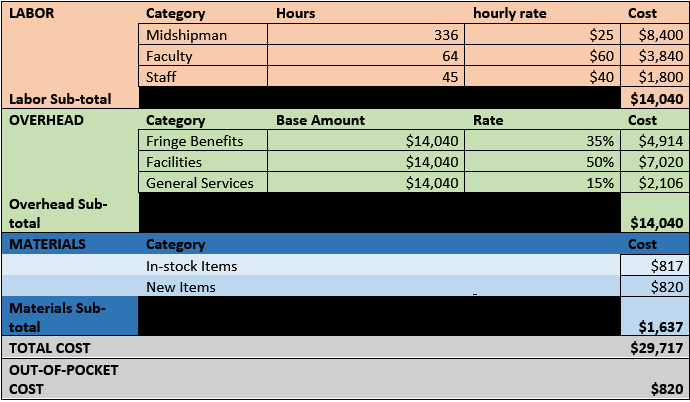
\includegraphics[width=0.8\columnwidth]{\myroot/figures/BUDGET_ew495report.png}
%\end{center}
%\label{table-budget}
%%just insert the table here as a figure... saved as a png
%\end{table}
%
%
%I have purchased and recieved all items that cover the originally proposed \$570 new item cost with the exception of a second additional Crazyflie 2.1 that was originally budgeted for, but I have not requested it yet for my research as I don't predict I will need it considering I have four old Crazyflie 2.0 models to use in addtion to the new 2.1 model I obtained with research funds. The increase in the total out-of-pocket cost is due to an approximately \SI{50}{\percent} increase added on to my original anticipated budget to account for any last-minute must-haves such as a battery charger that can charge multiple Crazyflies at once (will become more applicable as I get into more hardware testing). The in-stock item cost is derived from an approximated worth of \$198 for each of the four Crazyflie 2.0's that I'm using, as well as an additional \$25 for the use of old OptiTrack markers and the 3D printed rotor-guards. %\section{Discussion}



\section*{Acknowledgements}
I would like to thank Professor Clark for providing example \Canna\ trajectories to utilize for my research. 
%Additionally thanks to many members of USNA's faculty including Professor Piper and Professor Dawkins \would be more appropriate to add after next semester I think.

\bibliographystyle{IEEEtran}
\bibliography{IEEEabrv,\myroot/references/marcello}




%\clearpage
%\appendix
%\renewcommand{\figurename}{Supplementary Figure}
%\renewcommand{\thefigure}{S\arabic{figure}}
%\section{Timeline}
\label{sec:appA}

\begin{enumerate}
\item \textbf{Add Item 0. Get turnover from Canlas, Cuniff, exercise stuff to know we can fly, can talk to optitrack, and that you have a laptop available with all software planned to be used.}

\item Simulation
\begin{enumerate}
\item Familiarize myself with simulation capabilities.
\begin{enumerate}
\item Test all demos (1 week)
 \item Adapt some variables to see how the simulated results respond (1 week)
\item Upload model of the Crazyflie quadrotor to the simulation to be used for accurate simulation data. (1-3 days) 
\end{enumerate}

\item Create a desired path for the Crazyflies to fly.
\begin{enumerate}
\item Choose 3 different desired flight shapes and adapt simulation code to take them in as the desired flight path for the quadrotor. (1 week)
\item Run simulation tests and error calculations. Debug any issues with simulation. (1-2 weeks)
\item Plot all position, velocity, and accelerations vs. time (both linear and rotational on all 3 axis). (1-2 days)
\end{enumerate}

\item Test hummingbird trajectories in simulation.
\begin{enumerate}
\item Upload hummingbird dive trajectories into simulation. (3 days)
 \item Run simulation and plot position, velocity, and acceleration data vs. time for all 3 axes in both the linear and rotational frames. (2 days)
\item Conduct error calculations between the desired trajectory and the simulated trajectory of the quadrotor. (1 week)
\item Determine acceptable region of error, and determine a maximum theoretical performance for the quadrotor as a measure of how fast the quadrotor is able to complete the maneuver as compared to the hummingbird. (1 week)
\end{enumerate}
\end{enumerate}
 
\item Proof of Concept Demonstration
\begin{enumerate}
\item Purchase new Crazyflie and supporting materials
\begin{enumerate}
\item Create online shopping cart pdf of all materials: Crazyflie, extra blades, extra battery, more OptiTrack markers, etc. (3 days)
\item Create RQ forms and ITPR forms (\textbf{Marcello}\footnote{I've done the first ones as examples for you. You're doing all the others.}) (1 week).
\end{enumerate}

\item Obtain manual control of a Crazyflie with remote control.
\begin{enumerate}
\item Configure Crazyradio and obtain positive connection to the Crazyflie using Crazyflie PC client software. (1-2 days)
\item Connect controller to laptop and configure manual controls to Mode 2 (1 day)
\item Conduct takeoff/landing procedures. (1 day)
\item Fly a rough 3D pattern using manual control. (1 day)
\end{enumerate}

\item Obtain flight data using OptiTrack
\begin{enumerate}
\item Set up OptiTrack system to recognize Crazyflie as a rigid body. (3 days)
\item Run sample code to log flight data. (3 days)
\item Manually fly the Crazyflie and obtain flight data. (3 days)
\item Plot position, velocity, and acceleration data vs. time for all 3 axes in both the linear and rotational frames in \MATLAB. (3 days)
\end{enumerate}

\item Fly the Crazyflie Autonomously
\begin{enumerate}
\item Read about ROS and develop python proficiency (4 months, concurrent)
\item Develop/Utilize currently existing control algorithm architecture to autonomously control the Crazyflie through the input of specified waypoints with associated position, velocity, and (orientation?) information. (1-3 weeks)
\item Execute autonomous control and collect flight data using OptiTrack (1 week)
\item Plot position, velocity, and acceleration data vs. time for all 3 axes in both the linear and rotational frames in \MATLAB. (3 days)
\item Conduct error calculations between the desired trajectory and the actual flight trajectory data collected from the OptiTrack system. (1 week)
\item Present experimental findings (1 month).
\end{enumerate}

\end{enumerate}
\end{enumerate}

Total estimated time to completion: \SI{24}{weeks}.


  


\begin{IEEEbiography}[{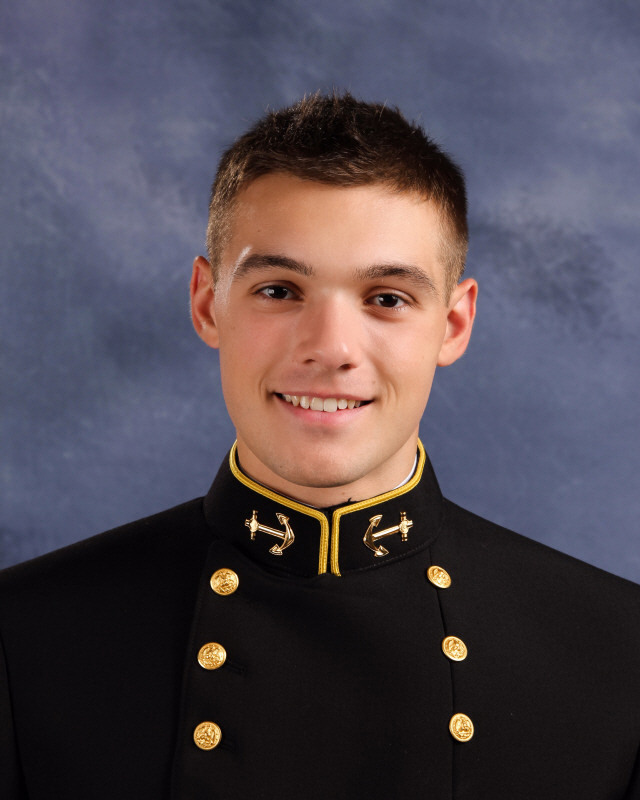
\includegraphics[width=1in,height=1.25in,clip,keepaspectratio]{\myroot/figures/M203876.jpg}}]{Ethan Marcello} is a midshipman at the United States Naval Academy majoring in Robotics and Control Engineering. Upon graduation, will attend graduate school at Northeastern University.  He has service selected Surface Warfare Officer with the Engineering Duty Officer option. 
\end{IEEEbiography}

%
%\begin{IEEEbiography}[{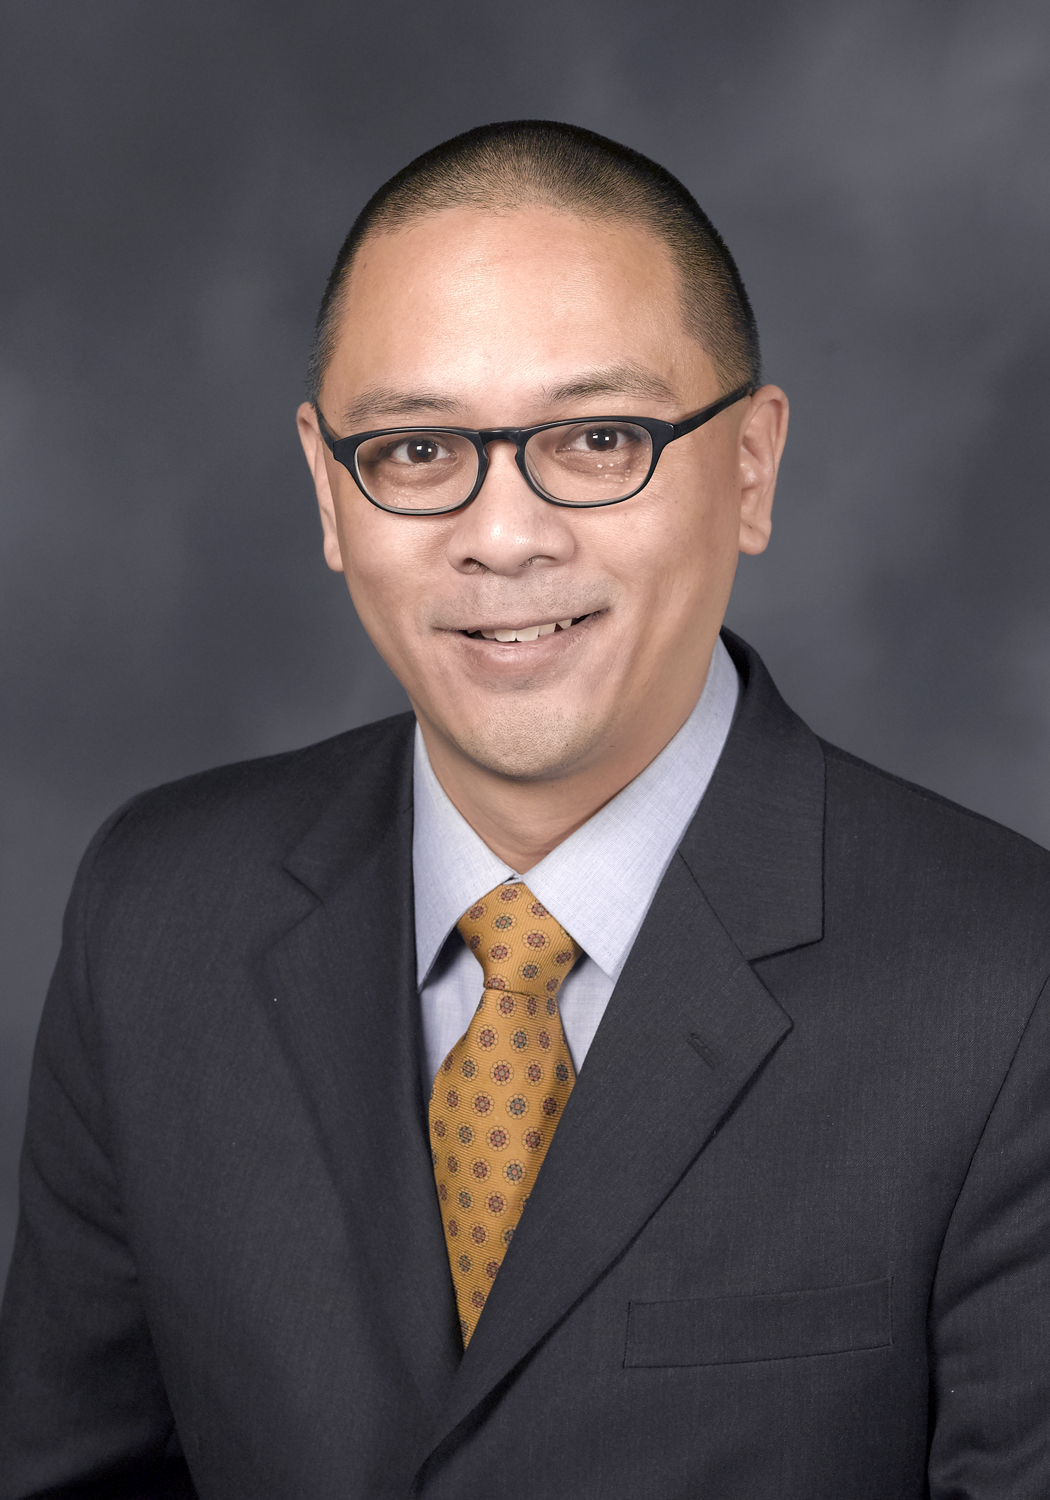
\includegraphics[width=1in,height=1.25in,clip,keepaspectratio]{\myroot/figures/evangelista_d_prof.jpg}}]{Dennis Evangelista} raises guide dog puppies. 
%\end{IEEEbiography}

\end{document}